%%%%%%%%%%%%%%%%%%%%%%%%%%%%%%%%%%%%%%%%%
% Beamer Presentation
% LaTeX Template
% Version 1.0 (10/11/12)
%
% This template has been downloaded from:
% http://www.LaTeXTemplates.com
%
% License:
% CC BY-NC-SA 3.0 (http://creativecommons.org/licenses/by-nc-sa/3.0/)
%
%%%%%%%%%%%%%%%%%%%%%%%%%%%%%%%%%%%%%%%%%

%----------------------------------------------------------------------------------------
%	PACKAGES AND THEMES
%----------------------------------------------------------------------------------------

\documentclass{beamer}

\mode<presentation> {

% The Beamer class comes with a number of default slide themes
% which change the colors and layouts of slides. Below this is a list
% of all the themes, uncomment each in turn to see what they look like.

%\usetheme{default}
%\usetheme{AnnArbor}
%\usetheme{Antibes}
%\usetheme{Bergen}
%\usetheme{Berkeley}
%\usetheme{Berlin}
%\usetheme{Boadilla}
%\usetheme{CambridgeUS}
%\usetheme{Copenhagen}
%\usetheme{Darmstadt}
%\usetheme{Dresden}
%\usetheme{Frankfurt}
%\usetheme{Goettingen}
%\usetheme{Hannover}
%\usetheme{Ilmenau}
%\usetheme{JuanLesPins}
%\usetheme{Luebeck}
\usetheme{Madrid}
%\usetheme{Malmoe}
%\usetheme{Marburg}
%\usetheme{Montpellier}
%\usetheme{PaloAlto}
%\usetheme{Pittsburgh}
%\usetheme{Rochester}
%\usetheme{Singapore}
%\usetheme{Szeged}
%\usetheme{Warsaw}

% As well as themes, the Beamer class has a number of color themes
% for any slide theme. Uncomment each of these in turn to see how it
% changes the colors of your current slide theme.

%\usecolortheme{albatross}
%\usecolortheme{beaver}
%\usecolortheme{beetle}
%\usecolortheme{crane}
%\usecolortheme{dolphin}
%\usecolortheme{dove}
%\usecolortheme{fly}
%\usecolortheme{lily}
%\usecolortheme{orchid}
%\usecolortheme{rose}
%\usecolortheme{seagull}
%\usecolortheme{seahorse}
%\usecolortheme{whale}
%\usecolortheme{wolverine}

%\setbeamertemplate{footline} % To remove the footer line in all slides uncomment this line
%\setbeamertemplate{footline}[page number] % To replace the footer line in all slides with a simple slide count uncomment this line

%\setbeamertemplate{navigation symbols}{} % To remove the navigation symbols from the bottom of all slides uncomment this line
}

\usepackage{graphicx} % Allows including images
\usepackage{booktabs} % Allows the use of \toprule, \midrule and \bottomrule in tables
\usepackage{subcaption}

%----------------------------------------------------------------------------------------
%	TITLE PAGE
%----------------------------------------------------------------------------------------

\title[Vector-Host Dynamics]{Modeling the Dynamics of Vector-Host Interactions in Avian Communities: Eastern Equine Encephalitis virus as a model system} % The short title appears at the bottom of every slide, the full title is only on the title page

\author[Tim Muller]{\emph{Timothy Muller}}
% Your name
\institute[ORST] % Your institution as it will appear on the bottom of every slide, may be shorthand to save space
{
Oregon State University \\ % Your institution for the title page
Medlock Lab \\
\medskip
\textit{mullert@onid.orst.edu} % Your email address
}
\date{\today} % Date, can be changed to a custom date

\begin{document}

\begin{frame}
\titlepage % Print the title page as the first slide
\end{frame}

%\begin{frame}
%\frametitle{Overview} % Table of contents slide, comment this block out to remove it
%\tableofcontents % Throughout your presentation, if you choose to use \section{} and \subsection{} commands, these will automatically be printed on this slide as an overview of your presentation
%\end{frame}

%----------------------------------------------------------------------------------------
%	PRESENTATION SLIDES
%----------------------------------------------------------------------------------------

%------------------------------------------------
%\section{First Section} % Sections can be created in order to organize your presentation into discrete blocks, all sections and subsections are automatically printed in the table of contents as an overview of the talk
%------------------------------------------------


\begin{frame}
\frametitle{Populations}
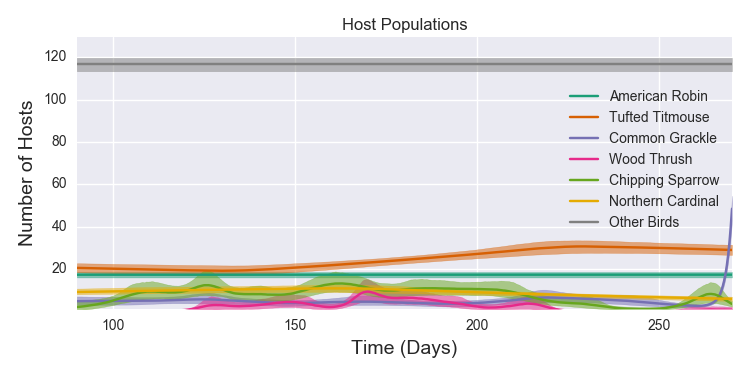
\includegraphics[width=\linewidth]{total_populations.png}
\end{frame}

\begin{frame}
\frametitle{Infections}
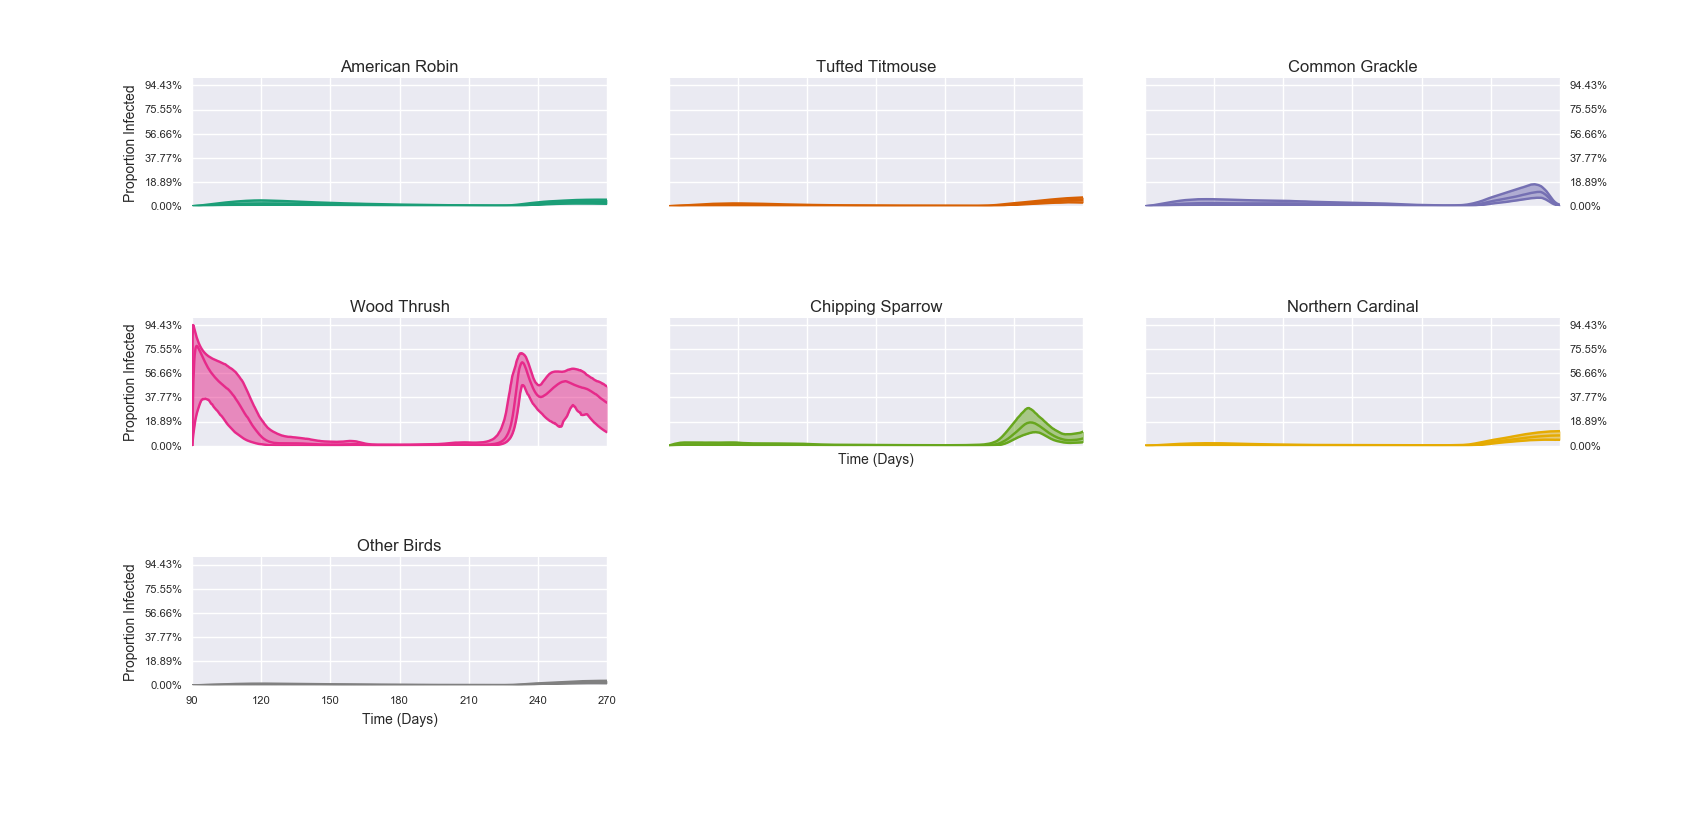
\includegraphics[width=\linewidth]{total_infections.png}
\end{frame}

\begin{frame}
\frametitle{Feeding Index}
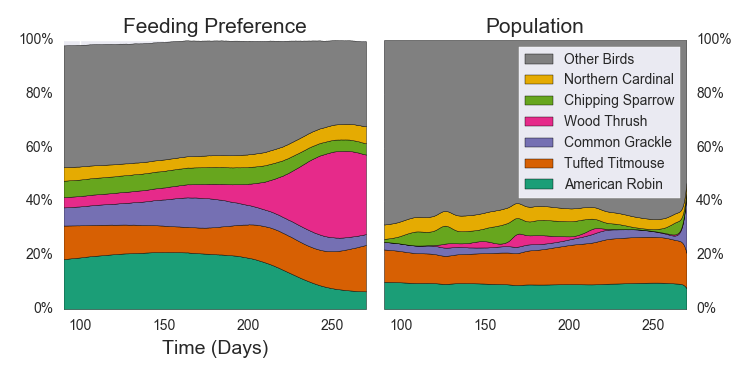
\includegraphics[width=\linewidth]{total_feeding_index.png}
\end{frame}

\begin{frame}
\frametitle{Species Examination}
\begin{itemize}
\item Want to examine the impact feeding preference has on infection
\item We combine a selected species with other birds, recreate the splines, and then re-simulate the ODE with the same parameter values
\end{itemize}
\end{frame}
%----------------------------------------------------------------------------------------

\begin{frame}
\frametitle{Feeding Index Comparisons}
\begin{figure}
\begin{subfigure}{0.48\textwidth}
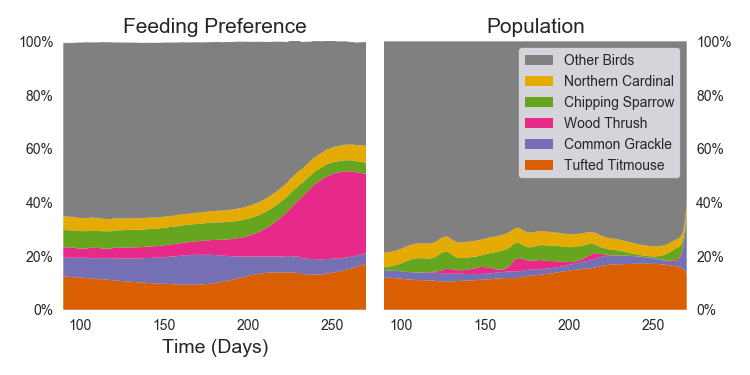
\includegraphics[width=\linewidth]{[0,6]_feedingindex.png}
\caption{American Robin Combined} \label{fig:a}
\end{subfigure}\hspace*{\fill}
\begin{subfigure}{0.48\textwidth}
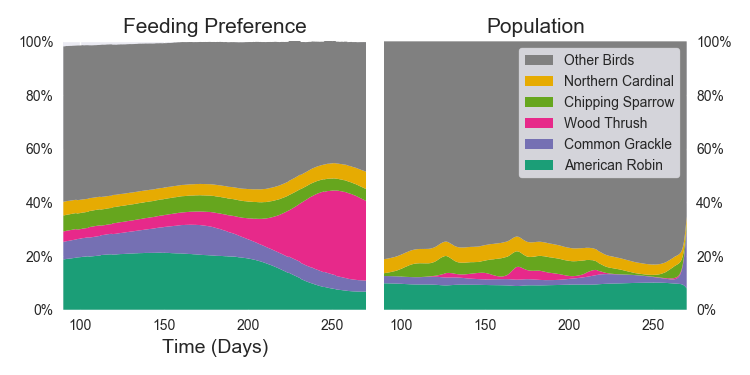
\includegraphics[width=\linewidth]{[1,6]_feedingindex.png}
\caption{Tufted Titmouse Combined} \label{fig:b}
\end{subfigure}

\medskip
\begin{subfigure}{0.48\textwidth}
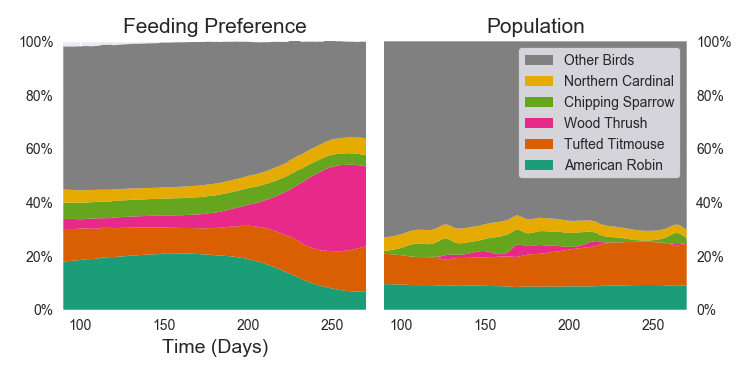
\includegraphics[width=\linewidth]{[2,6]_feedingindex.png}
\caption{Common Grackle Combined} \label{fig:c}
\end{subfigure}\hspace*{\fill}
\begin{subfigure}{0.48\textwidth}
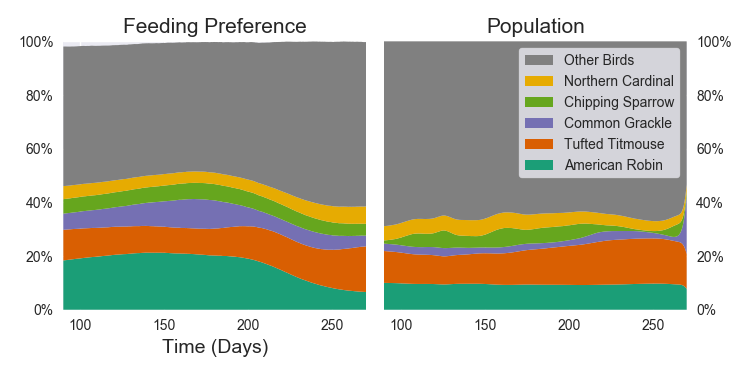
\includegraphics[width=\linewidth]{[3,6]_feedingindex.png}
\caption{Wood Thrush Combined} \label{fig:c}
\end{subfigure}
\end{figure}
\end{frame}

\begin{frame}
\frametitle{Feeding Index Comparisons Cont.}
\begin{figure}
\begin{subfigure}{0.48\textwidth}
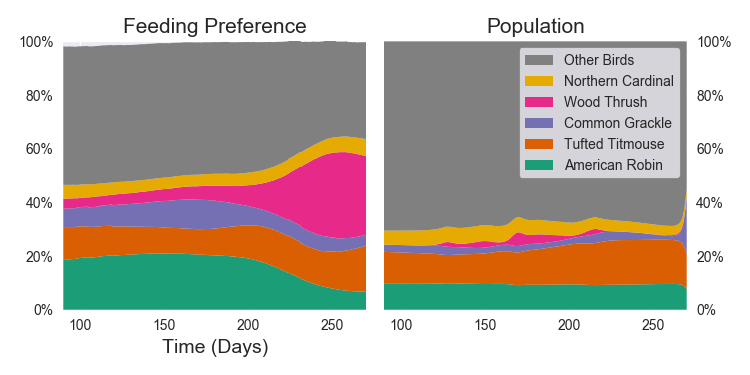
\includegraphics[width=\linewidth]{[4,6]_feedingindex.png}
\caption{Chipping Sparrow Combined} \label{fig:e}
\end{subfigure}\hspace*{\fill}
\begin{subfigure}{0.48\textwidth}
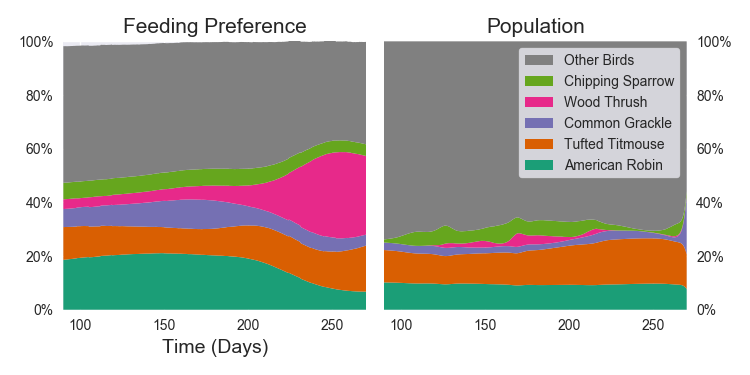
\includegraphics[width=\linewidth]{[5,6]_feedingindex.png}
\caption{Northern Cardinal Combined} \label{fig:g}
\end{subfigure}
\end{figure}
\end{frame}




\begin{frame}
\frametitle{Results}
\begin{center}
\begin{tabular}{ |c|c| } 
 \hline
 Species Combined & Percent Infected \\ [0.5ex] 
 \hline\hline
 \hline
 None & 15.2\% \\ 
 American Robin & 13.1\% \\ 
 Tufted Titmouse  & 15.6\% \\
 Common Grackle &  17.3\%      \\
 Wood Thrush &  \textbf{1.2\%}   \\
 Chipping Sparrow &  17.4\%   \\
 Northern Cardinal & 15.5\%    \\ 
 \hline
\end{tabular}
\end{center}
\end{frame}

\begin{frame}
\frametitle{American Robin Combined Infections}
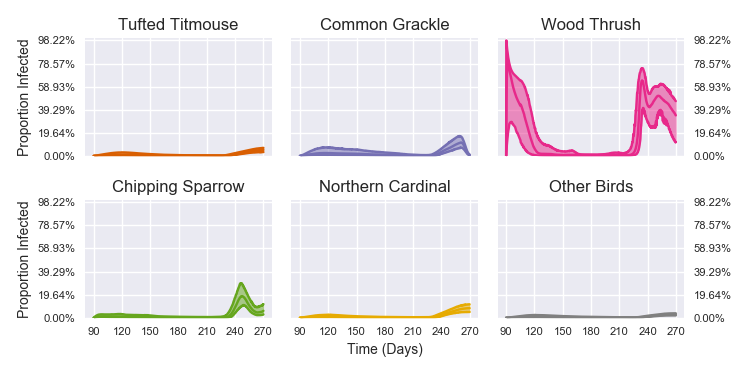
\includegraphics[width=\linewidth]{[0,6]_infections.png}
\end{frame}

\begin{frame}
\frametitle{Tufted Titmouse Combined Infections}
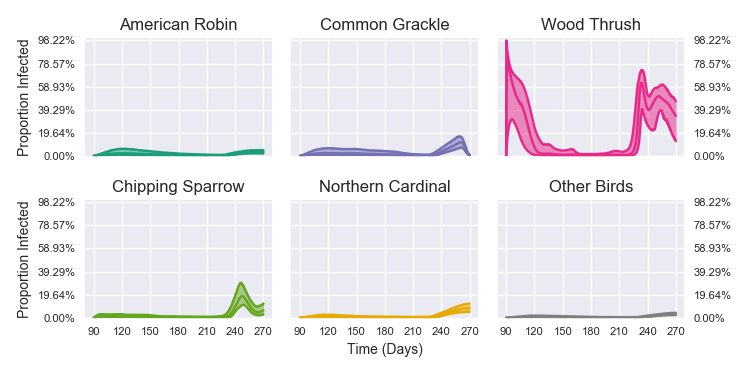
\includegraphics[width=\linewidth]{[1,6]_infections.png}
\end{frame}

\begin{frame}
\frametitle{Common Grackle Combined Infections}
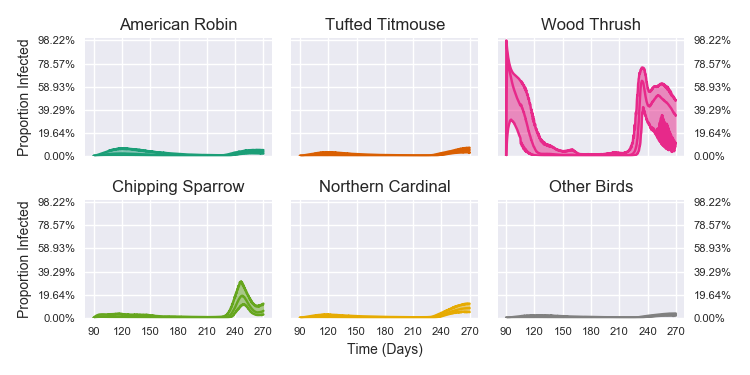
\includegraphics[width=\linewidth]{[2,6]_infections.png}
\end{frame}

\begin{frame}
\frametitle{Wood Thrush Combined Infections}
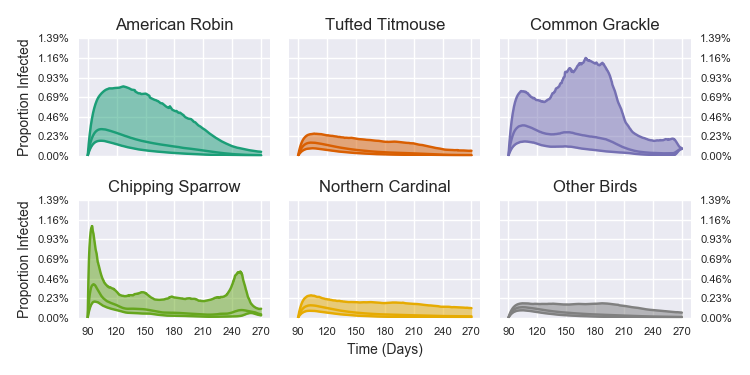
\includegraphics[width=\linewidth]{[3,6]_infections.png}
\end{frame}

\begin{frame}
\frametitle{Chipping Sparrow Combined Infections}
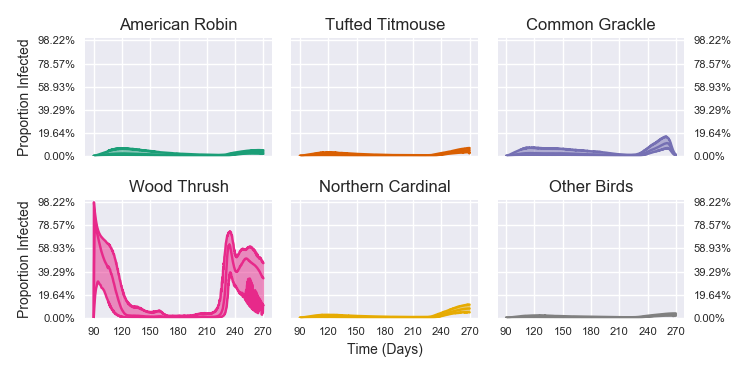
\includegraphics[width=\linewidth]{[4,6]_infections.png}
\end{frame}

\begin{frame}
\frametitle{Northern Cardinal Combined Infections}
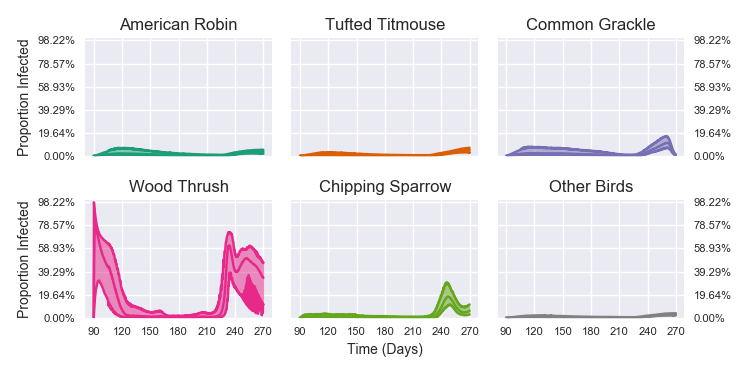
\includegraphics[width=\linewidth]{[5,6]_infections.png}
\end{frame}


\end{document}